\documentclass[UTF8]{ctexart}

\title{电子技术基础实验第十一周实验报告}

\author{王磊\quad2022012972}

\date{\today}

\usepackage{geometry}
\geometry{a4paper,scale=0.8}

\usepackage{graphicx}
\usepackage{subfigure}
\usepackage{float}

\usepackage{amsmath}

\usepackage{listings}
\usepackage{xcolor}
\usepackage{framed}
\usepackage{placeins}
\lstdefinestyle{verilogStyle}{
    language=verilog,
    basicstyle=\ttfamily,
    keywordstyle=\color{blue},
    commentstyle=\color{green},
    stringstyle=\color{red},
    numbers=left,
    numberstyle=\tiny\color{gray},
    breaklines=true,
    showstringspaces=false,
    columns = fixed,
    basewidth = 0.5em,
    captionpos=b,
}
\newcommand{\subsubsubsection}[1]{\paragraph{#1}\mbox{}\\}
\setcounter{secnumdepth}{4} % how many sectioning levels to assign numbers to
\setcounter{tocdepth}{4} % how many sectioning levels to show in ToC
%设置段落间距
\setlength{\parskip}{0.5em}
%令小标题左对齐
\CTEXsetup[format={\Large\bfseries}]{section}
%首行不缩进
\setlength{\parindent}{0pt}
\begin{document}
\maketitle
\section{模块设计}
\subsection{16位正弦数据生成}
使用matlab生成用于初始化ROM的mif文件,其中存储了256个16位的正弦数据,代码如图\ref{fig:matlab_code}所示。
\begin{figure}[!ht]
    \centering
    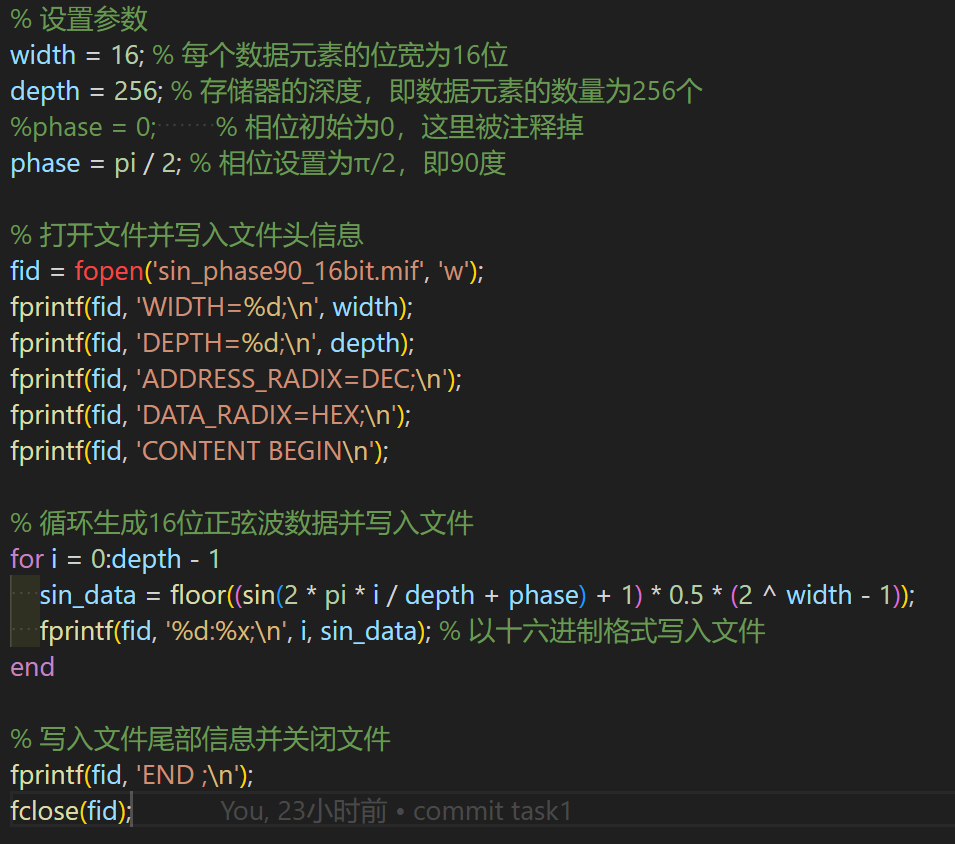
\includegraphics[width=0.8\textwidth]{matlab_code.png};

    \caption{matlab代码}
    \label{fig:matlab_code};
\end{figure}

生成的mif文件内容如图\ref{fig:mif}所示。
\begin{figure}[!ht]
    \centering
    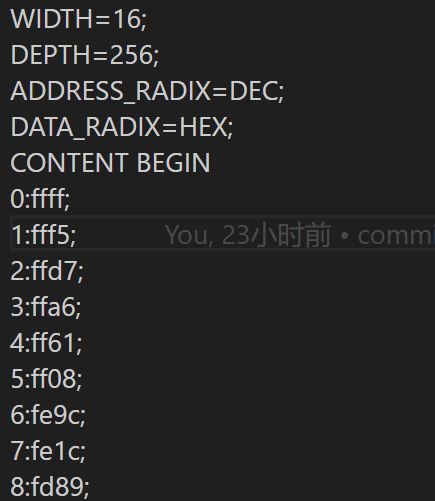
\includegraphics[width=0.8\textwidth]{mif.png};

    \caption{mif文件内容}
    \label{fig:mif};
\end{figure}

\subsection{实现60个16位数据加帧头发送}
\subsubsection{顶层模块}
顶层模块代码如下:
\begin{framed}
    \begin{lstlisting}[style=verilogStyle]
// This module is the top-level module for transmitting UART frames.
// It includes various sub-modules for address generation, data generation, and UART transmission.

`include "addr_tx_en.v" // Include module for address and transmit enable generation.
`include "sin_16_rom.v" // Include module for generating sine wave data.
`include "fre_div.v" // Include module for clock frequency division.
`include "uart_byte_controller.v" // Include module for byte-level UART transmission control.
`include "uart_2byte_controller_withoutHeader.v" // Include module for 2-byte UART transmission control without header.
`include "uart_tx_byte.v" // Include module for UART byte transmission.

module uart_frame_transmit_top (
    input  clk, // Clock input
    input  rst, // Reset input
    output sci_tx // UART transmit output
);

    wire clk_div_addr; // Clock divided address signal
    fre_div #(25'd12500) uut1 ( // Instantiate frequency divider module
        .clk(clk),
        .rst(rst),
        .clk_div_addr(clk_div_addr)
    );

    wire [7:0] addr; // Address signal
    wire send_en; // Transmit enable signal
    wire [15:0] data_out; // Output data signal

    addr_tx_en uut2 ( // Instantiate address and transmit enable module
        .clk_origin(clk),
        .clk(clk_div_addr),
        .rst(rst),
        .addr(addr),
        .data_temp(data_temp),
        .data_out(data_out),
        .tx_en(send_en)
    );

    wire [15:0] data_temp; // Temporary data signal
    sin_16_rom uut3 ( // Instantiate sine wave ROM module
        .address(addr),
        .clock(clk),
        .q(data_temp)
    );

    wire tx_en; // Transmit enable signal
    wire [7:0] tx_d; // Transmit data signal
    wire tx_done; // Transmission completion signal

    uart_2byte_controller_withoutHeader uut4 ( // Instantiate 2-byte UART controller module without header
        .clk(clk),
        .rst(rst),
        .send_en(send_en),
        .tx_en(tx_en),
        .tx_done(tx_done),
        .data(data_out),
        .tx_d(tx_d)
    );

    uart_tx_byte uut5 ( // Instantiate UART byte transmission module
        .clk(clk),
        .rst(rst),
        .tx_en(tx_en),
        .tx_done(tx_done),
        .rx_d(tx_d),
        .sci_tx(sci_tx)
    );

endmodule
\end{lstlisting}
\end{framed}
顶层模块的RTL图如图\ref{fig:top_rtl}所示。
\begin{figure}[!ht]
    \centering
    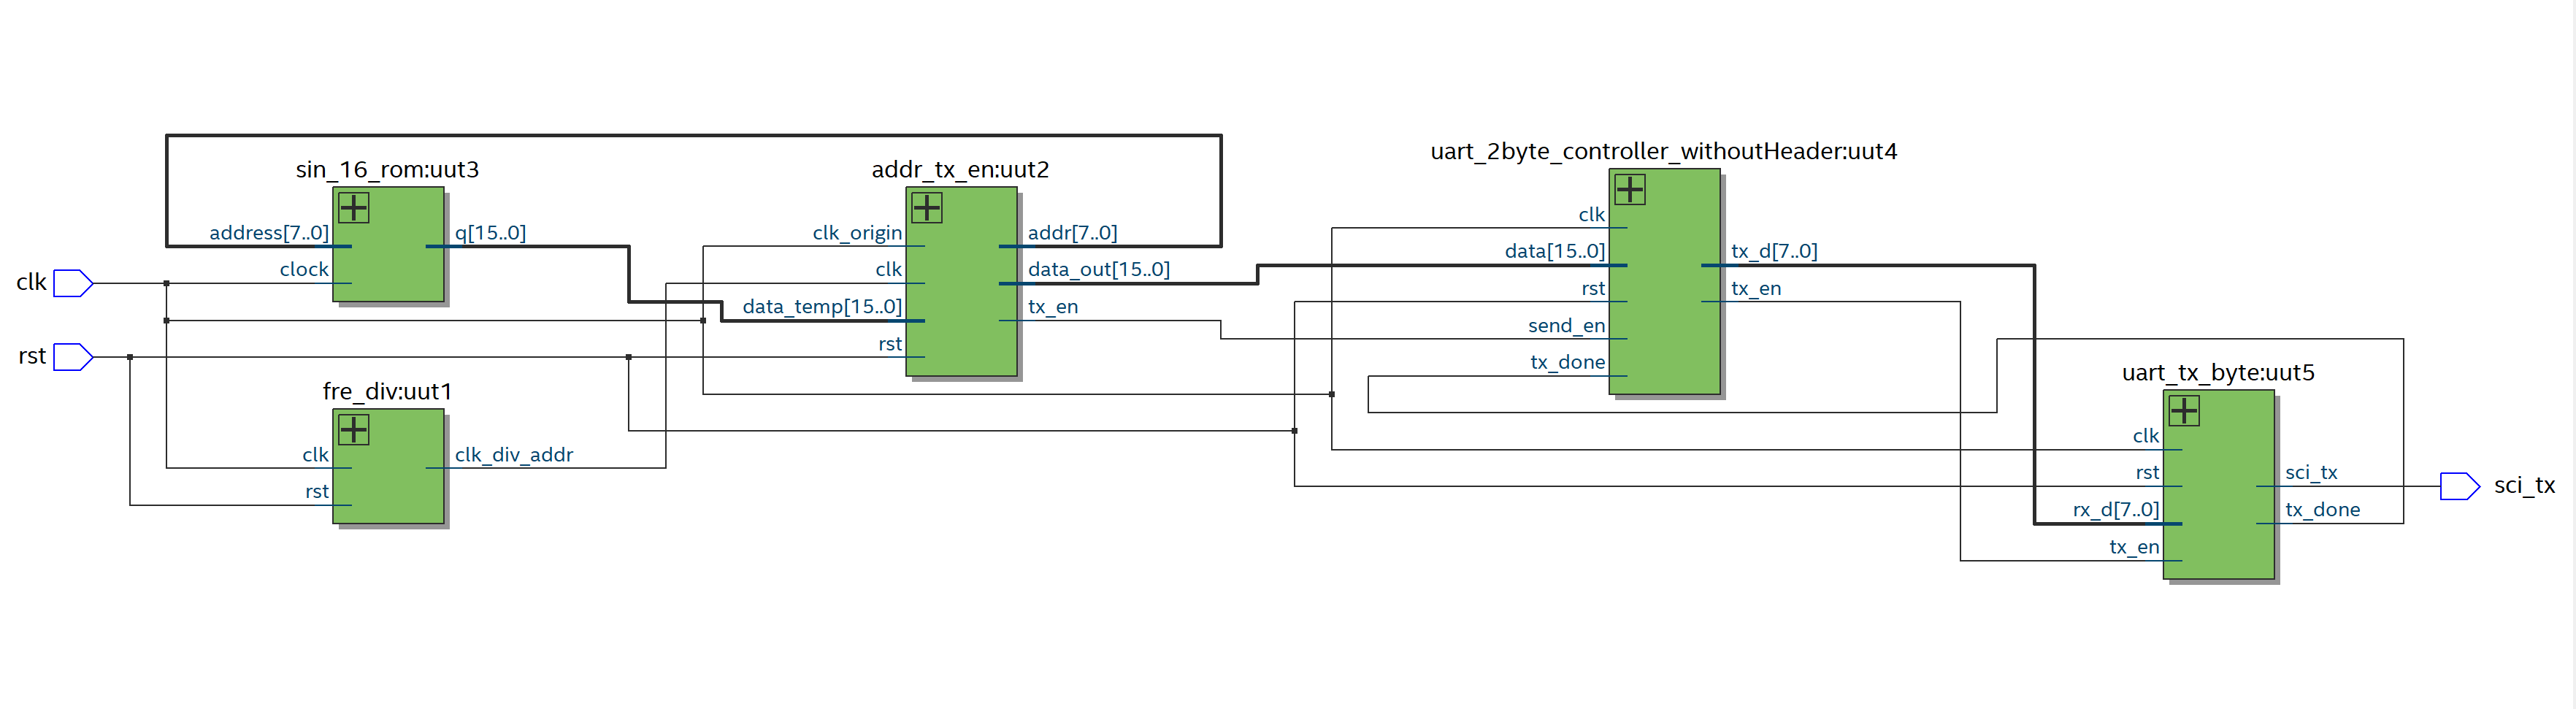
\includegraphics[width=0.8\textwidth]{top_rtl.png}

    \caption{顶层模块RTL图}
    \label{fig:top_rtl}
\end{figure}

具体的实现逻辑为:
\begin{enumerate}
    \item 通过分频模块分出1000Hz的时钟,用于触发地址模块。
    \item 地址模块每隔1ms产生一个地址,用于读取ROM中的数据。
    \item 地址模块同时具有计数与数据处理功能,从ROM中拿到的数据会先进入地址模块,按照任务要求加帧头帧尾后发送给16位UART发送模块。
\end{enumerate}

\subsubsection{地址模块}
该模块为本次任务的核心模块,代码如下:
\begin{framed}
    \begin{lstlisting}[style=verilogStyle]
// an idiot tried to write a counter in the state machine, and he failed.
// maybe put the counter in this module will work.

module addr_tx_en #(
    parameter FRAMENUM = 60
) (
    input clk,  // Clock input
    input clk_origin,  // Original clock input
    input rst,  // Reset input
    input [15:0] data_temp,  // Temporary data input
    output reg [15:0] data_out,  // Output data
    output reg [7:0] addr,  // Address output
    output reg tx_en  // Transmit enable output
);

    reg [5:0] frame_cnt;  // Frame counter

    always @(posedge clk, posedge rst) begin
        if (rst) begin
            addr <= 8'b00000000;  // Reset address
            frame_cnt <= 6'b000000;  // Reset frame counter
        end else begin
            if (addr == 8'b11111111) begin  // Check if address is at maximum value
                addr <= 8'b00000000;  // Reset address
            end else begin
                if (frame_cnt == FRAMENUM - 1) begin  // Check if frame counter is at maximum value
                    addr <= addr;  // Keep current address
                    data_out <= 16'h4545;  // Set output data
                    frame_cnt <= 6'b000000;  // Reset frame counter
                end else if (frame_cnt == 0) begin  // Check if frame counter is at minimum value
                    addr <= addr;  // Keep current address
                    data_out <= 16'h5353;  // Set output data
                    frame_cnt <= frame_cnt + 1'b1;  // Increment frame counter
                end else begin
                    addr <= addr + 1'b1;  // Increment address
                    data_out <= data_temp;  // Set output data
                    frame_cnt <= frame_cnt + 1'b1;  // Increment frame counter
                end
            end
        end
    end

    reg pulse1, pulse2, pulse3;  // Clock pulse signals
    wire clk_posedge;  // Positive edge clock signal

    always @(posedge clk_origin, posedge rst) begin
        if (rst) begin
            pulse1 <= 1'b0;  // Reset pulse1
            pulse2 <= 1'b0;  // Reset pulse2
            pulse3 <= 1'b0;  // Reset pulse3
        end else begin
            pulse1 <= clk;  // Assign pulse1 with clock input
            pulse2 <= pulse1;  // Assign pulse2 with pulse1
            pulse3 <= pulse2;  // Assign pulse3 with pulse2
        end
    end

    assign clk_posedge = pulse2 & ~pulse3;  // Calculate positive edge clock signal

    always @(posedge clk_origin, posedge rst) begin
        if (rst) begin
            tx_en <= 1'b0;  // Reset transmit enable
        end else begin
            if (clk_posedge) begin  // Check if positive edge clock signal is high
                tx_en <= 1'b1;  // Set transmit enable
            end else begin
                tx_en <= 1'b0;  // Reset transmit enable
            end
        end
    end

endmodule
    \end{lstlisting}
\end{framed}
本模块实现了一个计数器,用于记录发送的16位数据的个数。当计数器的值为0时,发送帧头;当计数器的值为59时,发送帧尾;其他情况下,发送数据。发送帧头帧尾的方式为:使用一个buffer先将ROM中的数读入备用,若需发送帧头或帧尾。扣留数据,使用帧头帧尾替换。同时让addr停止自增,确保数据不会中断。

\section{实现结果}
使用simulink接收串口数据,结果如图\ref{fig:simulink}所示。
\begin{figure}[!ht]
    \centering
    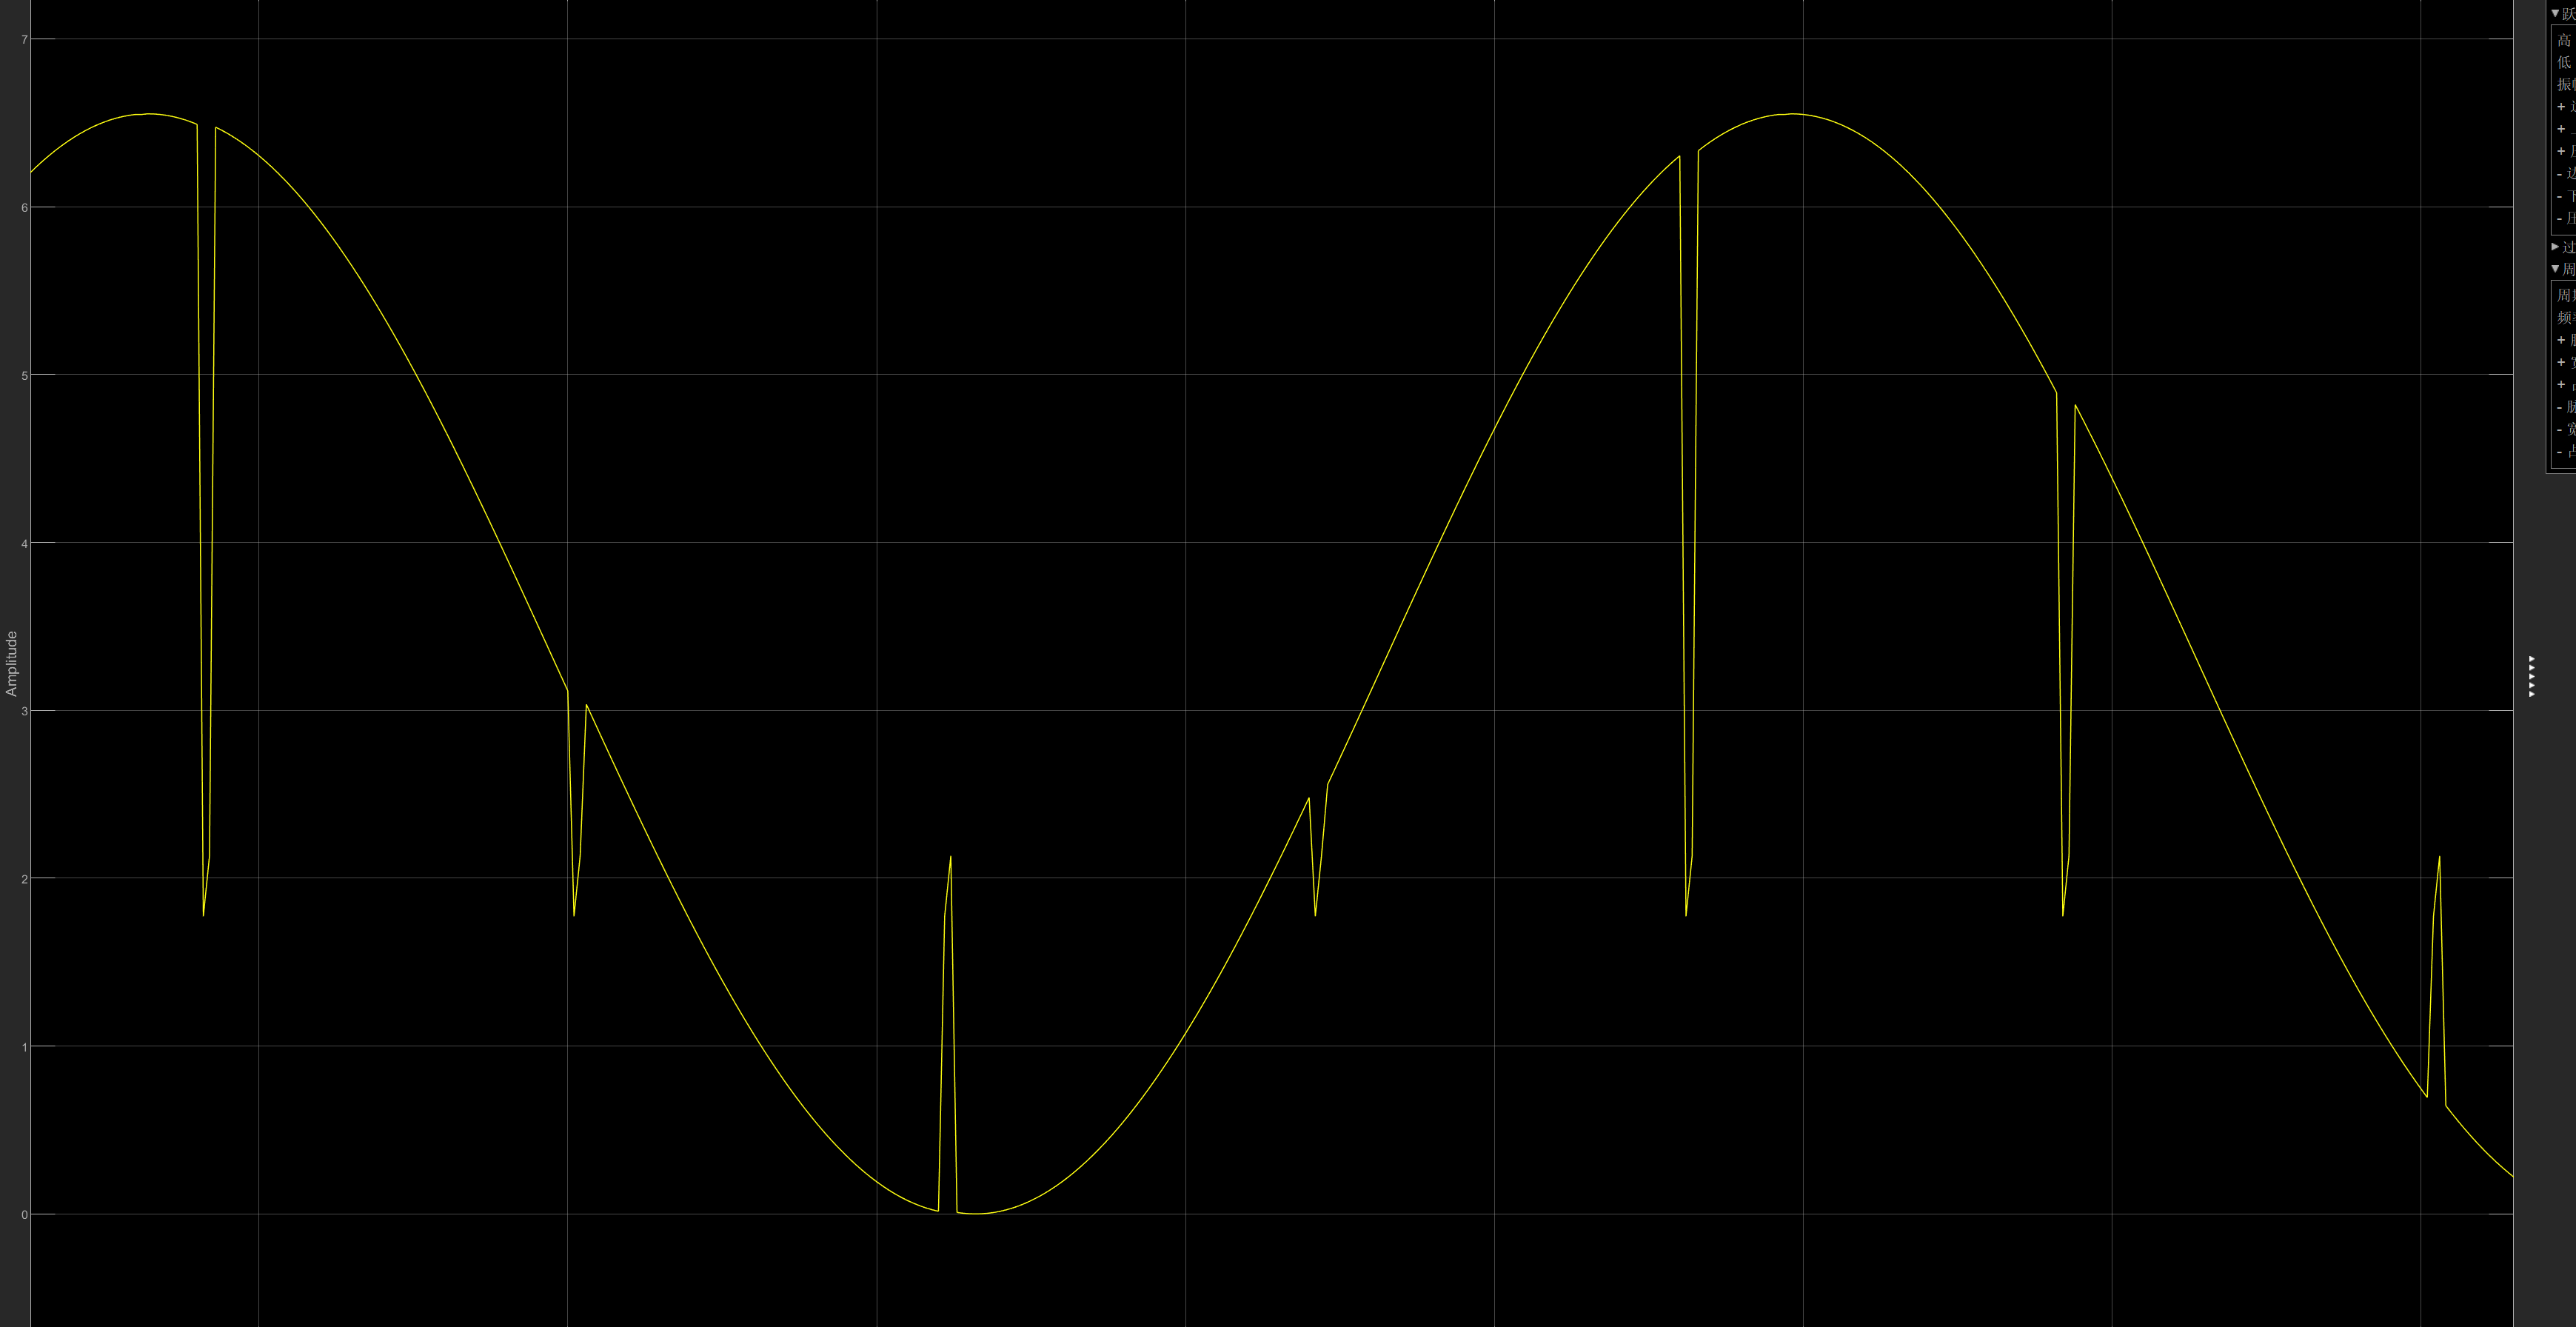
\includegraphics[width=0.8\textwidth]{simulink.png}
    \caption{simulink接收数据}
    \label{fig:simulink}
\end{figure}

其中定期产生的突刺为帧头帧尾,其他数据为正弦数据,可以看出帧头帧尾的发送不会影响正弦数据的完整性。






\end{document}